%!TEX root = paper.tex
%%%%%%%%%%%%%%%%%%%%%%%%%%%%%%%%%%%%%%%%%%%%%%%%%%%%%%%%%%%%%%%%%%%%%%%%%%%%%%%%
\section{Background}



%%%%%%%%%%%%%%%%%%%%%%%%%%%%%%%%%%%%%%%%%%%%%%%%%%%%%%%%%%%%%%%%%%%%%%%%%%%%%%%%
\subsection{Service Costs of Gaming Platforms}

Price Models of:

\paragraph{Steam and PC in General}

\paragraph{Consoles}

\paragraph{Historical Example: OnLinve}


\paragraph{Geforce Now}
\url{http://shield.nvidia.com/game-streaming-with-geforce-now}
Kosten

\$7.99/mo + 200\$/€++ Hardware

Started in parts of Europe in Q4/2015

Spieleangebot

\$x Spiele im Paket

 + weitere/neuere zusätzlich mit Einmalbetrag

Leistung
Bandbreite? 

\paragraph{Playstation Now}
Streaming von PS3 Spielen auf PS4 und andere Sony-Geräte (als Rückwärtskompatibiliätslösung)
Kosten

(US/UK only?) Deuschlandbeta seit ~Q4/2015

\$ /mo + 330\$/€ (PS4) oder Sony TV + Controller
Extrakosten/Tagesleihgebühren für bestimmte ``bessere'' Spiele




%%%%%%%%%%%%%%%%%%%%%%%%%%%%%%%%%%%%%%%%%%%%%%%%%%%%%%%%%%%%%%%%%%%%%%%%%%%%%%%%
\subsection{Platform Provider Costs}
Backend/Service Requirements and Demands

%%%%%%%%%%%%
\subsubsection{CAPEX}

\begin{itemize}
	\item Regionale Data Center
	\item Gaming Server (GPU-Enabled)
	\item Entwicklungskosten für Software-Plattform(?)
\end{itemize}

\paragraph{Hardware}

\url{https://www.nvidia.com/object/cloud-gaming-gpu-boards.html}
\url{https://www.nvidia.com/object/grid-technology.html}


%%%%%%%%%%%%
\subsubsection{OPEX}

\paragraph{Verkehrsvolumen}

\begin{itemize}
	\item Internetanbindung?
	\item Caching of basic resources is probably not applicable?
\end{itemize}

\paragraph{Serverlaufzeiten}

\begin{itemize}
	\item Energie
	\item Verschleiß
	\item Wartungs- und Betriebspersonal oder Anmietung
	\item Frage: Rechnet sich Anmietung von Ressourcen bei großen generischen Rechenzentren? Annahme nein, da man selbst ein großer Anbieter wäre u. die Margin wegfallen. Auf der anderen Seite gibt es Hardware die für Games im Serverbereich besser skalieren? Wenn ja, kann umso mehr kein generischer Anbieter die Lösung sein
\end{itemize}

\paragraph{Spiele-Lizenzen und -Adaptionskosten (?)}
Modelannahme: Kosten pro Nutzung (realistisch eher in Blöcken verrechnet)





%%%%%%%%%%%%%%%%%%%%%%%%%%%%%%%%%%%%%%%%%%%%%%%%%%%%%%%%%%%%%%%%%%%%%%%%%%%%%%%%
\subsection{Data}

Bereits Gesammelte Daten


%%%%%%%%%%%%
\subsubsection{Steam API + SteamSpy Datensätze+Graphen}
\url{https://github.com/mas-ude/steam-data-stats} Steam + SteamSpy REST API Datensammler + ein paar Graphplotter (und eher ergebnislose Clustering-Versuche); für sinnvolle Analsyen müsste man dazu aber viel häufiger Datensätze generieren. Beispielausgaben:

CDF der Preise auf Steam (Juli ‘15) \ref{fig:steam-prices}

\begin{figure}[!t]
	\centering
	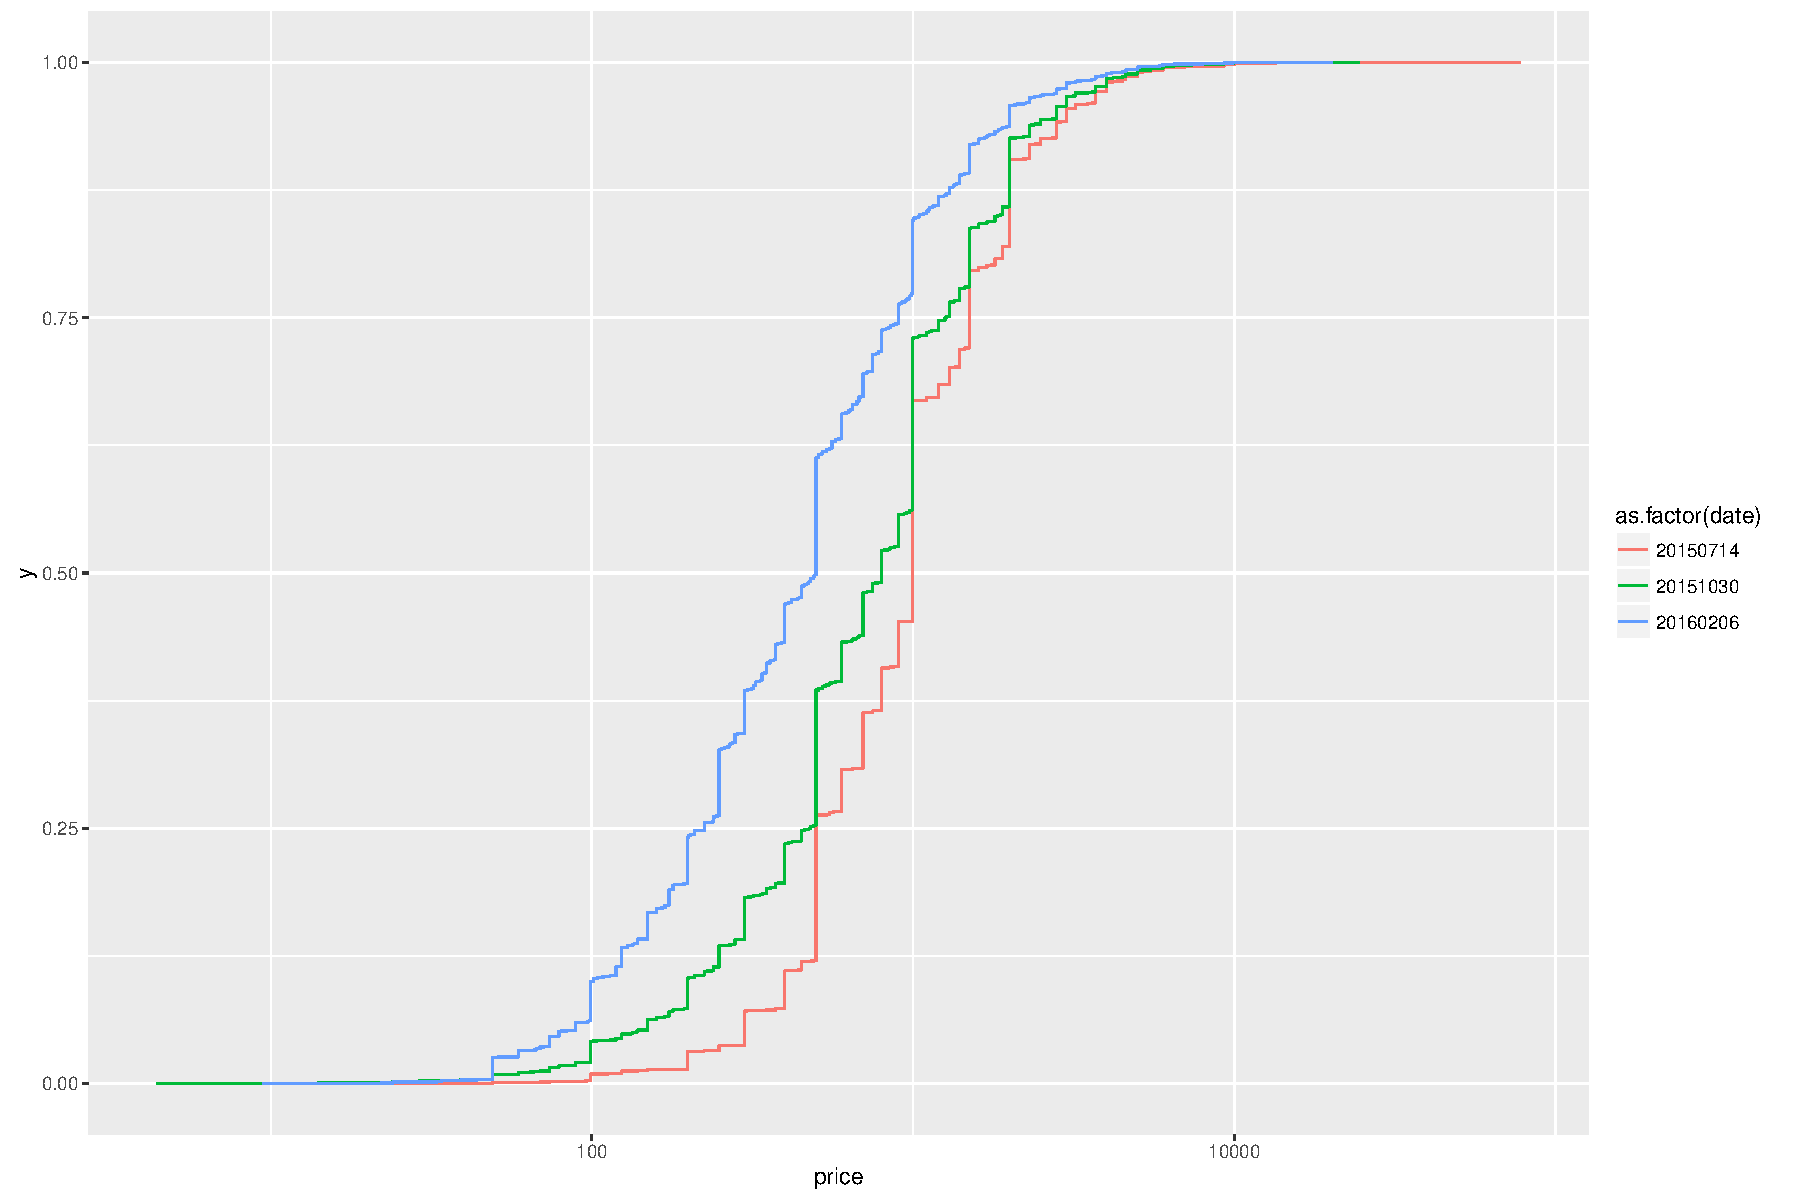
\includegraphics[width=1.0\columnwidth]{images/steam-prices.pdf}
	\caption{CDF of games on the steam platform at two distinct dates.}
\label{fig:steam-prices}
\end{figure}

Violinenplot der durchschnittlichen Spielzeit aufgeteilt auf unterschiedliche Preiskategorien. \ref{fig:steam-cost-vs-playtime-violin}

\begin{figure}[!t]
	\centering
	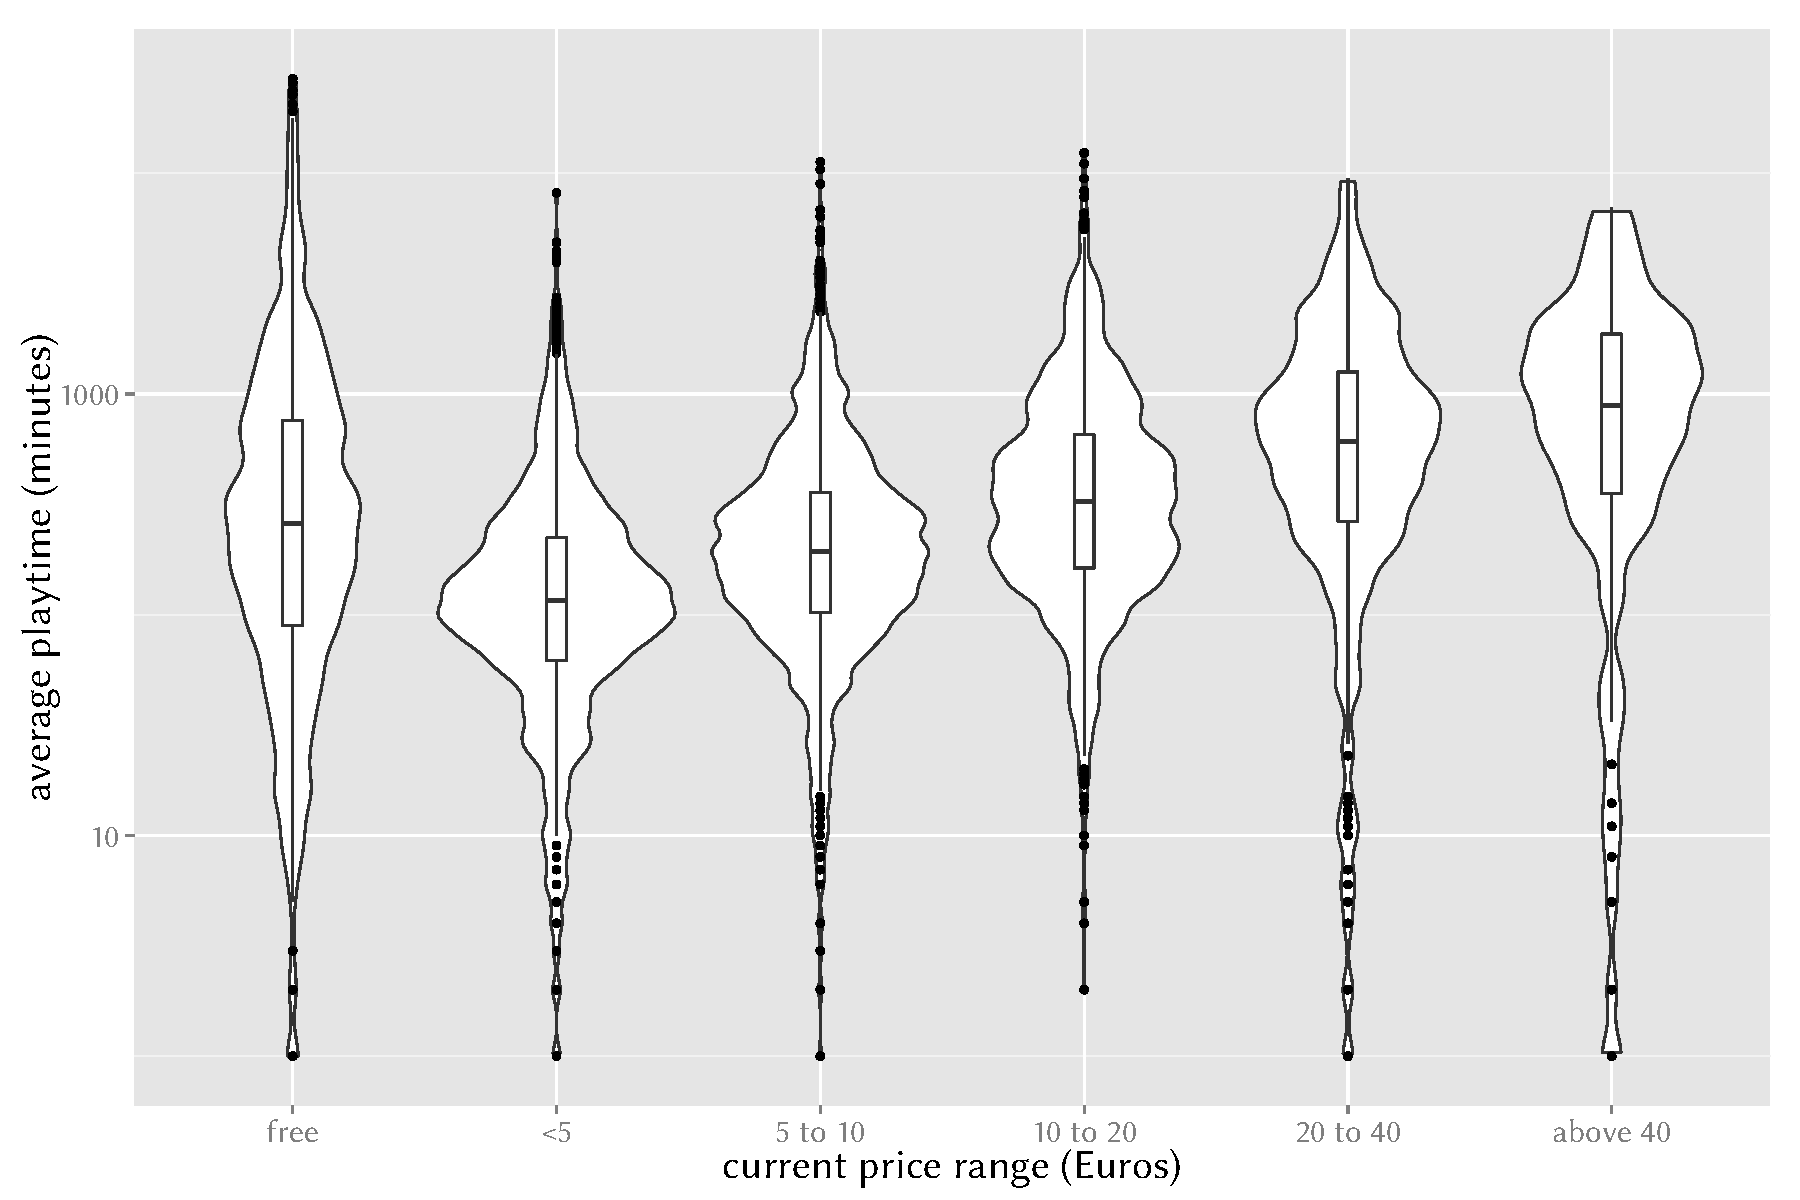
\includegraphics[width=1.0\columnwidth]{images/steam-cost-vs-playtime.pdf}
	\caption{Violin plot of the average playtime (as recorded by SteamSpy) of games categorized by their prices.}
\label{fig:steam-cost-vs-playtime-violin}
\end{figure}


%%%%%%%%%%%%
\subsubsection{platform-market-comparison/games-per-year.R}

 hat den ersten Versuch einer Nutzenrechnung für Spieler auf verschiedenen Plattformen. Script könnte leicht angepasst und erweitert werden. Beispielausgabe \ref{fig:gamesperyear-over-budget}, \ref{fig:steam-prices}

\begin{figure}[!t]
	\centering
	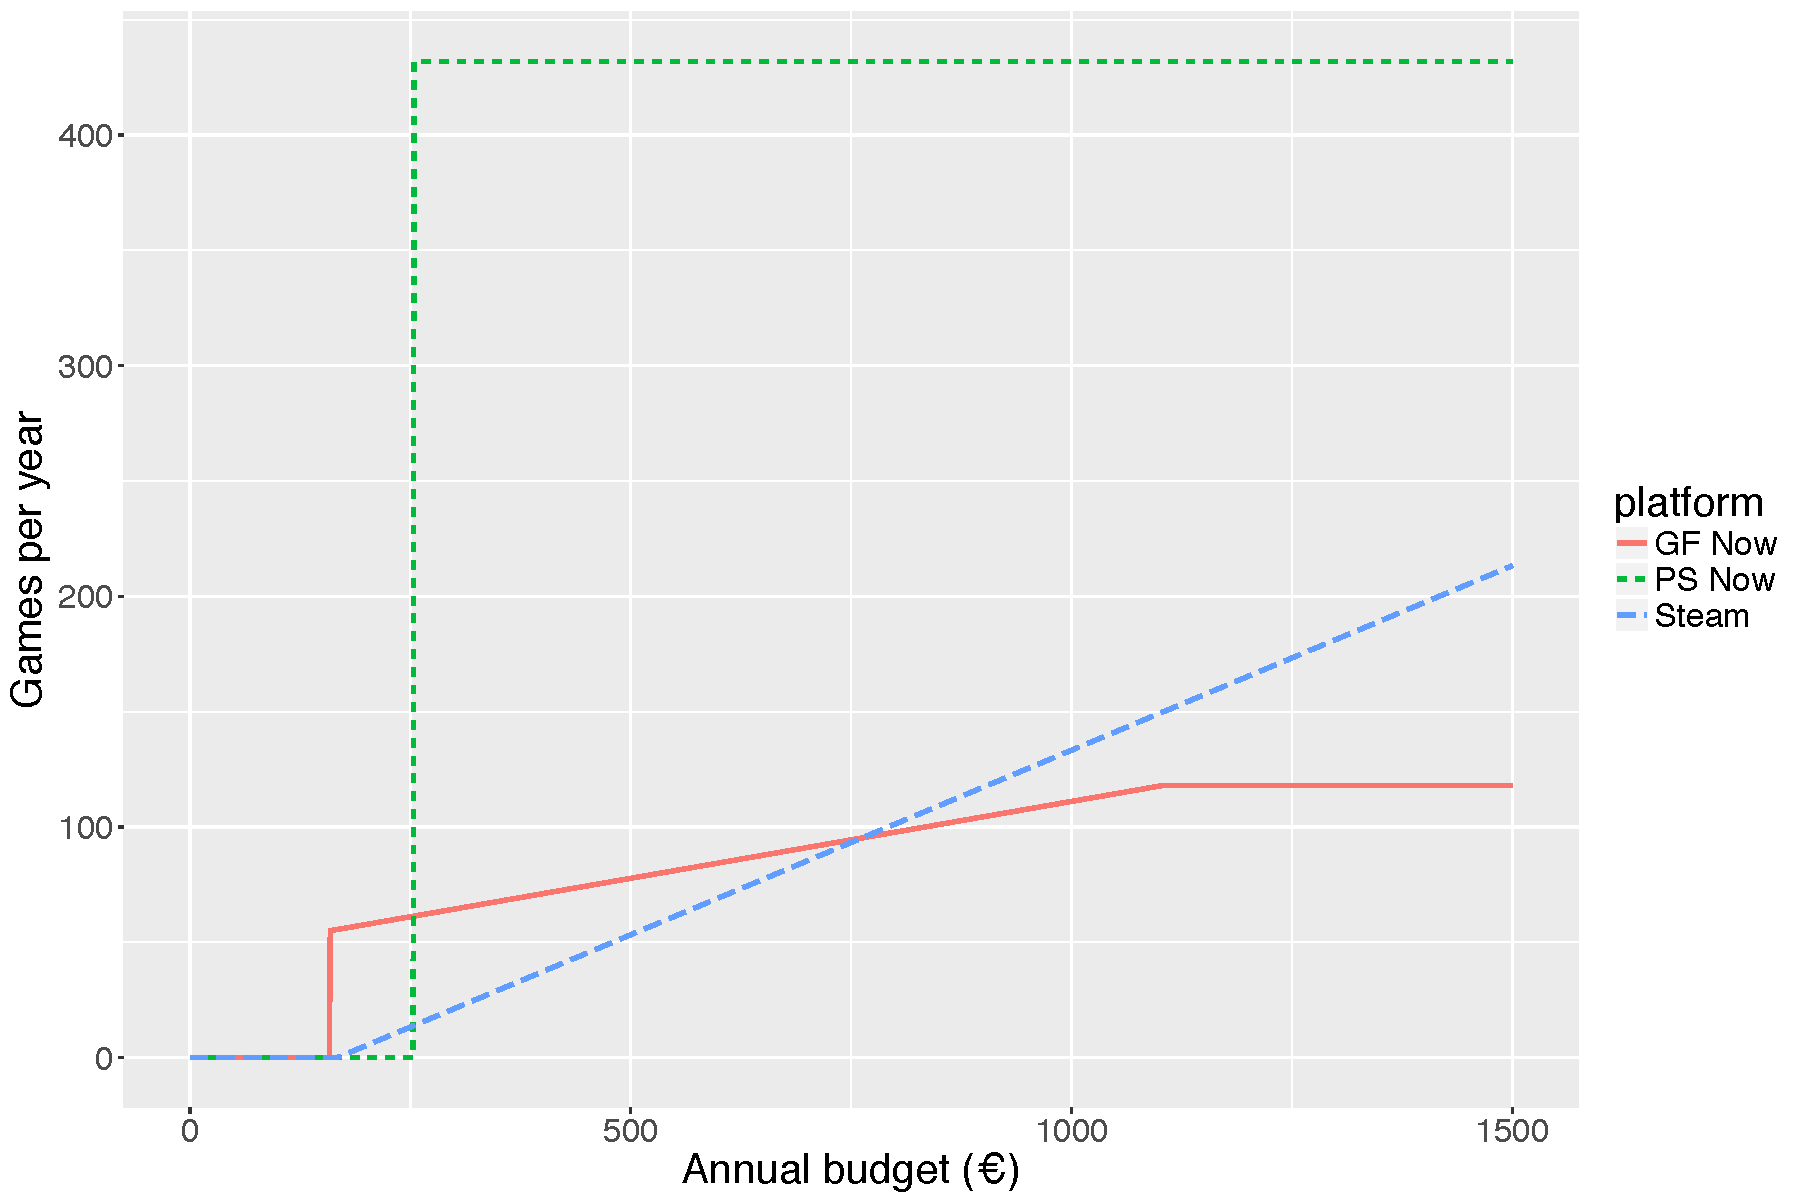
\includegraphics[width=1.0\columnwidth]{images/gamesperyear-over-budget.pdf}
	\caption{Models for several platforms showing the number of games per year that can be bought with a specific \$ budget.}
\label{fig:gamesperyear-over-budget}
\end{figure}

\begin{figure}[!t]
	\centering
	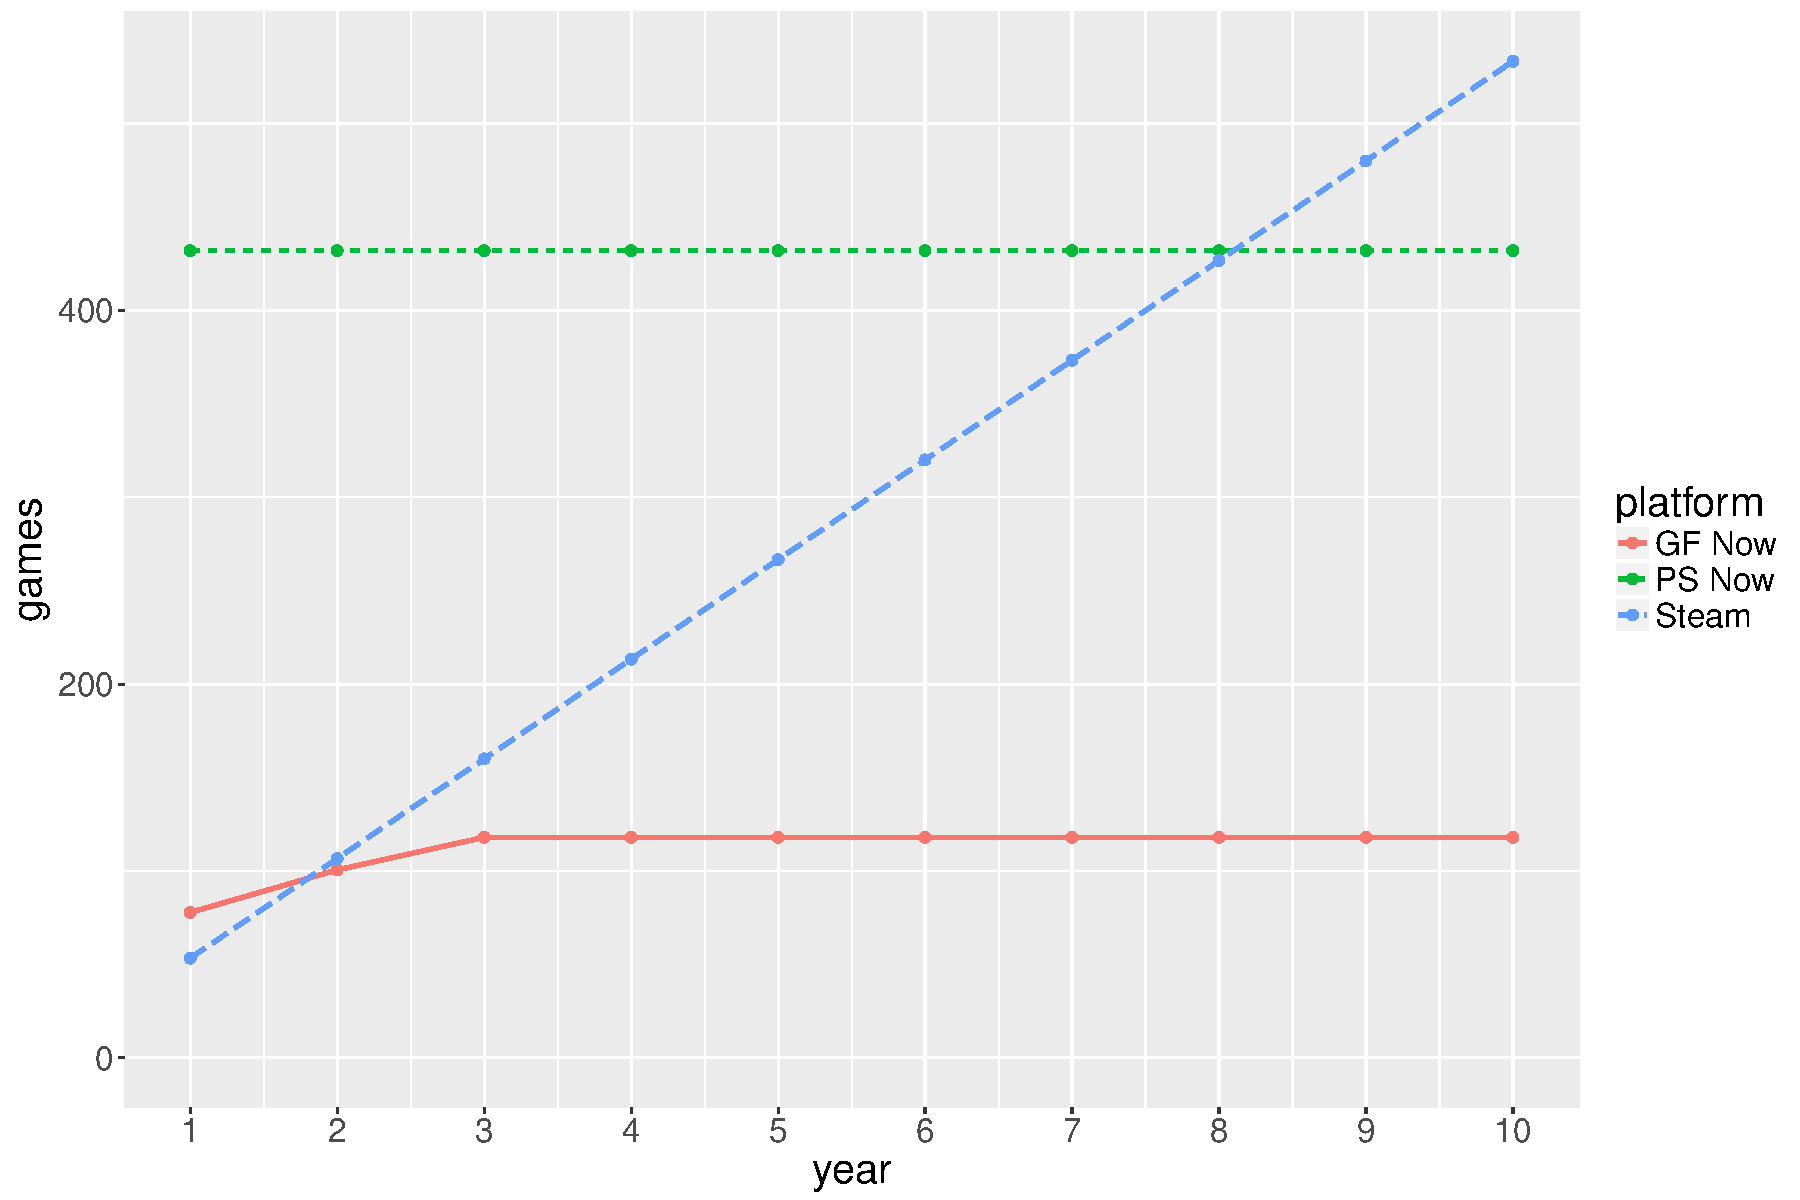
\includegraphics[width=1.0\columnwidth]{images/games-over-year.pdf}
	\caption{Models for several platforms showing the number of games that can be bought over the years subscribed to / using this service.}
\label{fig:games-over-years}
\end{figure}


\subsubsection{E2E Lag}
End-to-End Lag Model and Simulation in R. Now a standalone (submitted) paper at \url{https://github.com/mas-ude/onlinegame-lag-sim}. Can be referenced to argue the need for low E2E lag (meaning low network delay, but also the need for high fps).


%%%%%%%%%%%%
\subsubsection{Other Useful Data for Model Creation}

\begin{itemize}
	\item Game costs (current cost possible via Steam dataset; historic price data more difficult)
	\item Length of games (either via howlongtobeat dataset (via \url{https://github.com/mas-ude/gamelengths-scraper}), SteamSpy data, or could also additionally manually parse more Steam data)
	\item Gaming score/ratings/rankings (via Metacritic dataset (via \url{https://github.com/mas-ude/metacritic_scraper}), or might want to additionally scrape steam user review scores)
	\item Other popularity measures? (e.g. steamspy owner data?)
	\item Influence of E2E lag on games? (could be theorized indirectly through e2e lag sim + categorization attempts)
	\item Hardware requirements of games?
\end{itemize}

